\documentclass[10pt, aspectratio=43]{beamer}
\usepackage[utf8]{inputenc}
\usepackage[T1]{fontenc}
\usepackage{lmodern}
\usepackage{tcolorbox}
\usepackage{amsmath}
\usepackage{amsfonts}
\usepackage{amssymb}
\usepackage{amsthm}
\usepackage{stmaryrd}
\usepackage{caption}
\usepackage{appendixnumberbeamer}

\usepackage{algorithm,algpseudocode}
\usepackage{cancel}

\usepackage[document]{ragged2e}
\makeatletter
\DeclareOldFontCommand{\rm}{\normalfont\rmfamily}{\mathrm}
\DeclareOldFontCommand{\sf}{\normalfont\sffamily}{\mathsf}
\DeclareOldFontCommand{\tt}{\normalfont\ttfamily}{\mathtt}
\DeclareOldFontCommand{\bf}{\normalfont\bfseries}{\mathbf}
\DeclareOldFontCommand{\it}{\normalfont\itshape}{\mathit}
\DeclareOldFontCommand{\sl}{\normalfont\slshape}{\@nomath\sl}
\DeclareOldFontCommand{\sc}{\normalfont\scshape}{\@nomath\sc}
\makeatother

% \beamerdefaultoverlayspecification{<+->}

\newcommand{\X}{\mathsf{X}}
\newcommand{\Y}{\mathsf{Y}}
\renewcommand{\S}{\mathcal{S}}
\newcommand{\T}{\mathcal{T}}


\newcommand{\defeq}{\overset{\textsf{def}}{=}}

\usepackage{datetime}
\usepackage{nameref}

\usepackage{tikz}
\usepackage{pgfplots}

\usepackage{enumerate}
\usepackage{tikz}
\usetikzlibrary{decorations.pathreplacing}
\usetikzlibrary{patterns}
\usetikzlibrary{patterns.meta}
\usetikzlibrary{calc}

\usepackage{float}
\usepackage{multicol}

\definecolor{magenta}{rgb}{1.0, 0.0, 1.0}
\definecolor{alizarin}{rgb}{0.82, 0.1, 0.26}
\definecolor{antiquebrass}{rgb}{0.8, 0.58, 0.46}
\definecolor{darkturquoise}{rgb}{0.0, 0.81, 0.82}
\definecolor{darkpastelgreen}{rgb}{0.01, 0.75, 0.24}
\definecolor{darktangerine}{rgb}{1.0, 0.66, 0.07}
\definecolor{richcarmine}{rgb}{0.84, 0.0, 0.25}
\definecolor{majorelleblue}{rgb}{0.38, 0.31, 0.86}
\definecolor{magenta}{rgb}{1.0, 0.0, 1.0}
\definecolor{cobalt}{rgb}{0.0, 0.28, 0.67}
\definecolor{ferrarired}{rgb}{1.0, 0.11, 0.0}
\definecolor{battleshipgrey}{rgb}{0.52, 0.52, 0.51}
\definecolor{atomictangerine}{rgb}{1.0, 0.6, 0.4}
\definecolor{caribbeangreen}{rgb}{0.0, 0.8, 0.6}

\usetheme{EastLansing}

\setbeamertemplate{section in toc}[square]

\definecolor{cadmiumgreen}{rgb}{0.0, 0.42, 0.24}
\definecolor{airforceblue}{rgb}{0.36, 0.54, 0.66}
\definecolor{bondiblue}{rgb}{0.0, 0.58, 0.71}

\newtheorem*{conj*}{Conjecture}
\newtheorem*{lmm*}{Lemme}

\setbeamercovered{transparent}
\makeatother
\author{Benoît \textsc{Bompol}, Armand \textsc{Grenier}}
\subtitle{Combinatorial Optimization and Graph Theory}
\title[Directed hypergraph connectivity orientation]{\textsf{\textbf{Directed hypergraph connectivity augmentation by hyperarc re-orientations}}}
\date{Thursday, Nov 23rd 2023}

\pgfplotsset{compat=1.18}
\begin{document}
	\begin{frame}[plain]
		\maketitle
	\end{frame}
	
	\begin{frame}{Table of contents}
		\tableofcontents
	\end{frame}
	
	\section{Introduction}
	\subsection{Connectivity problems, characterisations}
	\begin{frame}{State of the art, goal of the article}
		\begin{itemize}
			\visible<2->{\item \textit{Nash-Williams}, 1960 :}
			\visible<2->{\begin{itemize}
					\item $G$ is $2k$-edge connected $\iff$ $G$ admits a $k$-arc-connected orientation.
			\end{itemize}}
			
			\visible<3->{\item \textit{Ito and al.}, 2023 : }
			\visible<3->{\begin{itemize}
					\item Algorithmic proof of \textit{Nash-Williams}, by flipping one arc at a time.
					\item Exhibiting a sequence of orientations such that :
					\begin{itemize}
						\item The arc-connectivity does not decrease, and the arc-connectivity of the last element of the sequence is $k$.
						\item The next orientation in the sequence can be obtained from the previous one by flipping exactly one arc.
						\item The sequence can be obtained in polynomial time (in the size of the directed graph).
					\end{itemize}
			\end{itemize}}
		\end{itemize}
		
		\visible<4->{Goal of the article : Expanding the result of \textbf{Ito and al.} to hypergraphs.\\}
		\visible<5->{Side note : This article generalise the results of \textbf{Ito and al.}, as directed graphs are special case of hypergraphs.}
	\end{frame}
	
	\subsection{Hypergraphs}
	\begin{frame}{Hypergraphs}    
		\begin{figure}[H]
			\centering
			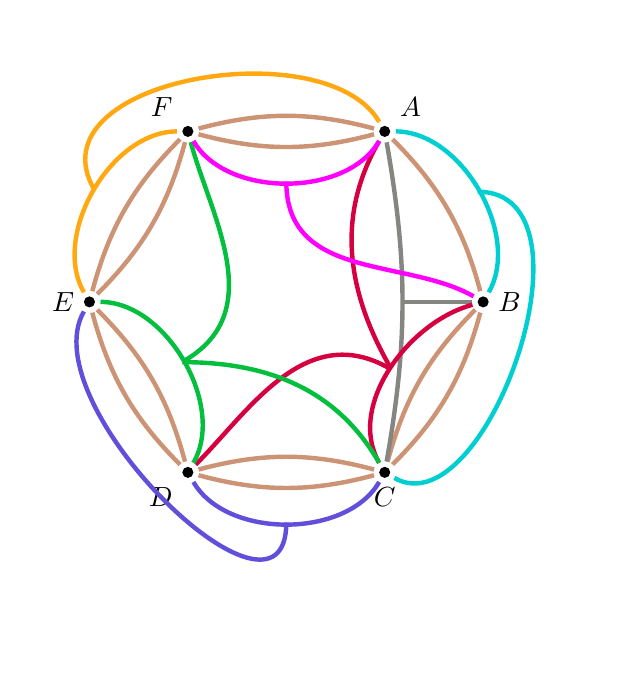
\begin{tikzpicture}
				\def\radius{2.5}
				\coordinate (A) at (60:\radius);
				\coordinate (B) at (0:\radius);
				\coordinate (C) at (300:\radius);
				\coordinate (D) at (240:\radius);
				\coordinate (E) at (180:\radius);
				\coordinate (F) at (120:\radius);
				
				\fill (A) circle (2pt); \node[above right=2pt] at (A) {$A$};
				\fill (B) circle (2pt); \node[right=2pt] at (B) {$B$};
				\fill (C) circle (2pt); \node[below=2pt] at (C) {$C$};
				\fill (D) circle (2pt); \node[below left=2pt] at (D) {$D$};
				\fill (E) circle (2pt); \node[left=2pt] at (E) {$E$};
				\fill (F) circle (2pt); \node[above left=2pt] at (F) {$F$};
				
				
				\visible<1->{
					\draw[ultra thick, antiquebrass, shorten <= 4pt, shorten >= 4pt] (A) to [out=-45, in=105] (B);
					\draw[ultra thick, antiquebrass, shorten <= 4pt, shorten >= 4pt] (B) to [out=-105, in=45] (C);
					\draw[ultra thick, antiquebrass, shorten <= 4pt, shorten >= 4pt] (C) to [out=195, in=-15] (D);
					\draw[ultra thick, antiquebrass, shorten <= 4pt, shorten >= 4pt] (D) to [out=135, in=-75] (E);
					\draw[ultra thick, antiquebrass, shorten <= 4pt, shorten >= 4pt] (E) to [out=75, in=-135] (F);
					\draw[ultra thick, antiquebrass, shorten <= 4pt, shorten >= 4pt] (F) to [out=15, in=165] (A);
				}
				
				\visible<4->{
					\draw[ultra thick, antiquebrass, shorten <= 4pt, shorten >= 4pt] (A) to [out=195, in=-15] (F);            \draw[ultra thick, antiquebrass, shorten <= 4pt, shorten >=4pt] (C) to [out=75, in=-135] (B);
					\draw[ultra thick, antiquebrass, shorten <= 4pt, shorten >= 4pt] (D) to [out=15, in=165] (C);
					\draw[ultra thick, antiquebrass, shorten <= 4pt, shorten >= 4pt] (E) to [out=-45, in=105] (D);
					\draw[ultra thick, antiquebrass, shorten <= 4pt, shorten >= 4pt] (F) to [out=-105, in=45] (E);
				}
				
				\visible<2->{
					% {AC -> B}
					\draw[ultra thick, battleshipgrey, shorten <= 4pt, shorten >= 4pt] (A) to [out=-80, in=80] node[pos=0.5] (ac) {} (C);
					\draw[ultra thick, battleshipgrey, shorten <= -4pt, shorten >= 4pt] (ac) to [out = 0, in = 180] (B);
				}
				
				
				\visible<4->{
					% {AB -> C}
					\draw[ultra thick, darkturquoise, shorten <= 4pt, shorten >= 4pt] (A) to [out=0, in=60] node[pos=0.5] (ab) {}   (B);
					\draw[ultra thick, darkturquoise, shorten <= -4pt, shorten >= 4pt] (ab) to [out = 0, in = -30] (C);
				}
				
				\visible<3->{
					% {ABC -> D}
					\draw[ultra thick, richcarmine, shorten <= 4pt, shorten >= 4pt] (B) to [out=195, in=120] node[pos=0.5] (bc) {} (C);
					\draw[ultra thick, richcarmine, shorten <= 4pt, shorten >= -4pt] (A) to [out=-120, in=120] (bc);
					\draw[ultra thick, richcarmine, shorten <= -4pt, shorten >= 4pt] (bc) to [out = 150, in = 45] (D);
				}
				
				\visible<4->{
					% {CD -> E}
					\draw[ultra thick, majorelleblue, shorten <= 4pt, shorten >= 4pt] (C) to [out=240, in=-60] node[pos=0.5] (cd) {} (D);
					\draw[ultra thick, majorelleblue, shorten <= -4pt, shorten >= 4pt] (cd) to [out = -90, in = -120] (E);
				}
				
				\visible<4->{
					% {CDE -> F}
					\draw[ultra thick, darkpastelgreen, shorten <= 4pt, shorten >= 4pt] (D) to [out=60, in=0] node[pos=0.5] (de) {}     (E);
					\draw[ultra thick, darkpastelgreen, shorten <= 4pt, shorten >= -4pt] (C) to [out=120, in=0] (de);
					\draw[ultra thick, darkpastelgreen, shorten <= -4pt, shorten >= 4pt] (de) to [out = 30, in = -75] (F);
				}
				
				\visible<4->{
					% {EF -> A}
					\draw[ultra thick, darktangerine, shorten <= 4pt, shorten >= 4pt] (E) to [out=120,in=180] node[pos=0.5] (ef) {} (F);
					\draw[ultra thick, darktangerine, shorten <= -4pt, shorten >= 4pt] (ef) to [out = 120, in = 120] (A);
				}
				
				\visible<4->{
					% {FA -> B}
					\draw[ultra thick, magenta, shorten <= 4pt, shorten >= 4pt] (F) to [out = -60, in = -120] node[pos=0.5] (fa) {}     (A);
					\draw[ultra thick, magenta, shorten <= -4pt, shorten >= 4pt] (fa) to [out = -90, in = 150] (B);
				}
			\end{tikzpicture}
		\end{figure}
	\end{frame}
	
	\begin{frame}{Degree of $\varnothing\not=\mathsf{X}\subsetneq V$}
		$d_{\mathcal{H}}(\mathsf{X})$ is the number of hyperedges intersecting both $\mathsf{X}$ and $V\setminus\mathsf{X}$.
		\begin{figure}[H]
			\centering
			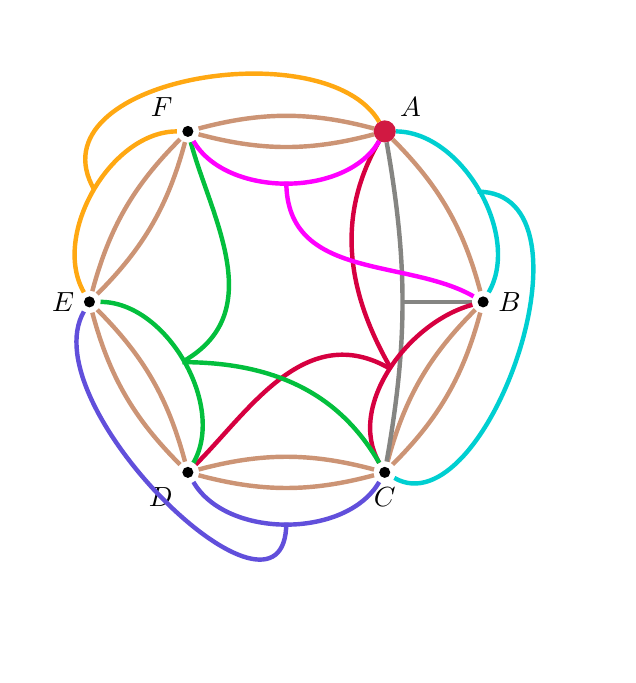
\begin{tikzpicture}
				\def\radius{2.5}
				\coordinate (A) at (60:\radius);
				\coordinate (B) at (0:\radius);
				\coordinate (C) at (300:\radius);
				\coordinate (D) at (240:\radius);
				\coordinate (E) at (180:\radius);
				\coordinate (F) at (120:\radius);
				
				\node[above right=2pt] at (A) {$A$}; \fill (A) circle (2pt); \visible<2->{\fill[alizarin] (A) circle (4pt);}
				\fill (B) circle (2pt); \node[right=2pt] at (B) {$B$};
				\fill (C) circle (2pt); \node[below=2pt] at (C) {$C$};
				\fill (D) circle (2pt); \node[below left=2pt] at (D) {$D$};
				\fill (E) circle (2pt); \node[left=2pt] at (E) {$E$};
				\fill (F) circle (2pt); \node[above left=2pt] at (F) {$F$};
				
				
				\visible<-2>{
					\draw[ultra thick, antiquebrass, shorten <= 4pt, shorten >= 4pt] (C) to [out=195, in=-15] (D);
					\draw[ultra thick, antiquebrass, shorten <= 4pt, shorten >= 4pt] (B) to [out=-105, in=45] (C);
					\draw[ultra thick, antiquebrass, shorten <= 4pt, shorten >= 4pt] (D) to [out=135, in=-75] (E);
					\draw[ultra thick, antiquebrass, shorten <= 4pt, shorten >= 4pt] (E) to [out=75, in=-135] (F);
					\draw[ultra thick, antiquebrass, shorten <= 4pt, shorten >=4pt] (C) to [out=75, in=-135] (B);
					\draw[ultra thick, antiquebrass, shorten <= 4pt, shorten >= 4pt] (D) to [out=15, in=165] (C);
					\draw[ultra thick, antiquebrass, shorten <= 4pt, shorten >= 4pt] (E) to [out=-45, in=105] (D);
					\draw[ultra thick, antiquebrass, shorten <= 4pt, shorten >= 4pt] (F) to [out=-105, in=45] (E);
				}
				
				\visible<-3>{
					\draw[ultra thick, antiquebrass, shorten <= 4pt, shorten >= 4pt] (A) to [out=-45, in=105] (B);
					\draw[ultra thick, antiquebrass, shorten <= 4pt, shorten >= 4pt] (A) to [out=195, in=-15] (F);
					\draw[ultra thick, antiquebrass, shorten <= 4pt, shorten >= 4pt] (F) to [out=15, in=165] (A);
				}
				
				\visible<-3>{
					% {AC -> B}
					\draw[ultra thick, battleshipgrey, shorten <= 4pt, shorten >= 4pt] (A) to [out=-80, in=80] node[pos=0.5] (ac) {} (C);
					\draw[ultra thick, battleshipgrey, shorten <= -4pt, shorten >= 4pt] (ac) to [out = 0, in = 180] (B);
					
					% {AB -> C}
					\draw[ultra thick, darkturquoise, shorten <= 4pt, shorten >= 4pt] (A) to [out=0, in=60] node[pos=0.5] (ab) {} (B);
					\draw[ultra thick, darkturquoise, shorten <= -4pt, shorten >= 4pt] (ab) to [out = 0, in = -30] (C);
					
					% {ABC -> D}
					\draw[ultra thick, richcarmine, shorten <= 4pt, shorten >= 4pt] (B) to [out=195, in=120] node[pos=0.5] (bc) {} (C);
					\draw[ultra thick, richcarmine, shorten <= 4pt, shorten >= -4pt] (A) to [out=-120, in=120] (bc);
					\draw[ultra thick, richcarmine, shorten <= -4pt, shorten >= 4pt] (bc) to [out = 150, in = 45] (D);
				}
				
				\visible<-2>{
					% {CD -> E}
					\draw[ultra thick, majorelleblue, shorten <= 4pt, shorten >= 4pt] (C) to [out=240, in=-60] node[pos=0.5] (cd) {} (D);
					\draw[ultra thick, majorelleblue, shorten <= -4pt, shorten >= 4pt] (cd) to [out = -90, in = -120] (E);
					
					% {CDE -> F}
					\draw[ultra thick, darkpastelgreen, shorten <= 4pt, shorten >= 4pt] (D) to [out=60, in=0] node[pos=0.5] (de) {} (E);
					\draw[ultra thick, darkpastelgreen, shorten <= 4pt, shorten >= -4pt] (C) to [out=120, in=0] (de);
					
					\draw[ultra thick, darkpastelgreen, shorten <= -4pt, shorten >= 4pt] (de) to [out = 30, in = -75] (F);
				}
				
				\visible<-3>{
					% {EF -> A}
					\draw[ultra thick, darktangerine, shorten <= 4pt, shorten >= 4pt] (E) to [out=120,in=180] node[pos=0.5] (ef) {} (F);
					\draw[ultra thick, darktangerine, shorten <= -4pt, shorten >= 4pt] (ef) to [out = 120, in = 120] (A);
					
					% {FA -> B}
					\draw[ultra thick, magenta, shorten <= 4pt, shorten >= 4pt] (F) to [out = -60, in = -120] node[pos=0.5] (fa) {}  (A);
					\draw[ultra thick, magenta, shorten <= -4pt, shorten >= 4pt] (fa) to [out = -90, in = 150] (B);
				}
				
			\end{tikzpicture}
		\end{figure}
	\end{frame}
	
	\begin{frame}{Orientation of an hypergraph}
		\begin{figure}[H]
			\centering
			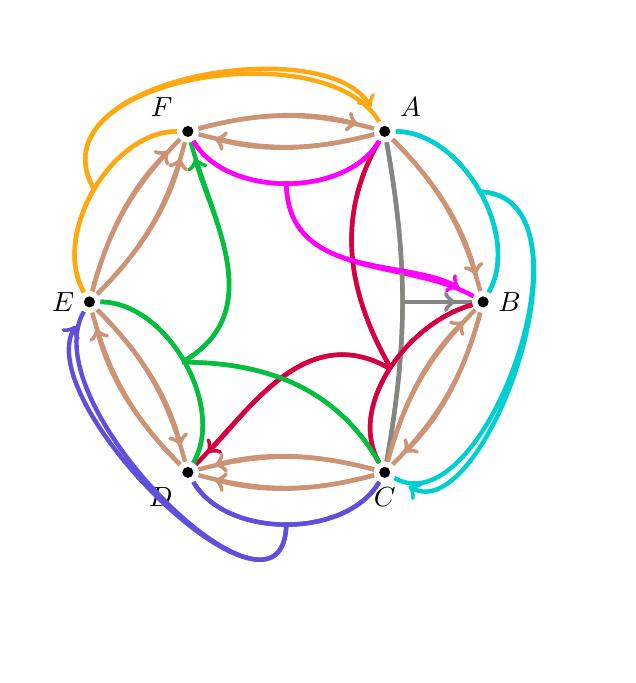
\begin{tikzpicture}
				\def\radius{2.5}
				\coordinate (A) at (60:\radius);
				\coordinate (B) at (0:\radius);
				\coordinate (C) at (300:\radius);
				\coordinate (D) at (240:\radius);
				\coordinate (E) at (180:\radius);
				\coordinate (F) at (120:\radius);
				
				\fill (A) circle (2pt); \node[above right=2pt] at (A) {$A$};
				\fill (B) circle (2pt); \node[right=2pt] at (B) {$B$};
				\fill (C) circle (2pt); \node[below=2pt] at (C) {$C$};
				\fill (D) circle (2pt); \node[below left=2pt] at (D) {$D$};
				\fill (E) circle (2pt); \node[left=2pt] at (E) {$E$};
				\fill (F) circle (2pt); \node[above left=2pt] at (F) {$F$};
				
				\visible<-1>{
					\draw[ultra thick, antiquebrass, shorten <= 4pt, shorten >= 4pt] (A) to [out=-45, in=105] (B);
					\draw[ultra thick, antiquebrass, shorten <= 4pt, shorten >= 4pt] (B) to [out=-105, in=45] (C);
					\draw[ultra thick, antiquebrass, shorten <= 4pt, shorten >= 4pt] (C) to [out=195, in=-15] (D);
					\draw[ultra thick, antiquebrass, shorten <= 4pt, shorten >= 4pt] (D) to [out=135, in=-75] (E);
					\draw[ultra thick, antiquebrass, shorten <= 4pt, shorten >= 4pt] (E) to [out=75, in=-135] (F);
					\draw[ultra thick, antiquebrass, shorten <= 4pt, shorten >= 4pt] (F) to [out=15, in=165] (A);
					\draw[ultra thick, antiquebrass, shorten <= 4pt, shorten >= 4pt] (A) to [out=195, in=-15] (F);
					
					
					% {AC -> B}
					\draw[ultra thick, battleshipgrey, shorten <= 4pt, shorten >= 4pt] (A) to [out=-80, in=80] node[pos=0.5] (ac) {} (C);
					\draw[ultra thick, battleshipgrey, shorten <= -4pt, shorten >= 4pt] (ac) to [out = 0, in = 180] (B);
					
					
					\draw[ultra thick, antiquebrass, shorten <= 4pt, shorten >=4pt] (C) to [out=75, in=-135] (B);
					\draw[ultra thick, antiquebrass, shorten <= 4pt, shorten >= 4pt] (D) to [out=15, in=165] (C);
					\draw[ultra thick, antiquebrass, shorten <= 4pt, shorten >= 4pt] (E) to [out=-45, in=105] (D);
					\draw[ultra thick, antiquebrass, shorten <= 4pt, shorten >= 4pt] (F) to [out=-105, in=45] (E);
					
					% {AB -> C}
					\draw[ultra thick, darkturquoise, shorten <= 4pt, shorten >= 4pt] (A) to [out=0, in=60] node[pos=0.5] (ab) {} (B);
					\draw[ultra thick, darkturquoise, shorten <= -4pt, shorten >= 4pt] (ab) to [out = 0, in = -30] (C);
					
					% {ABC -> D}
					\draw[ultra thick, richcarmine, shorten <= 4pt, shorten >= 4pt] (B) to [out=195, in=120] node[pos=0.5] (bc) {} (C);
					\draw[ultra thick, richcarmine, shorten <= 4pt, shorten >= -4pt] (A) to [out=-120, in=120] (bc);
					\draw[ultra thick, richcarmine, shorten <= -4pt, shorten >= 4pt] (bc) to [out = 150, in = 45] (D);
					
					% {CD -> E}
					\draw[ultra thick, majorelleblue, shorten <= 4pt, shorten >= 4pt] (C) to [out=240, in=-60] node[pos=0.5] (cd) {} (D);
					\draw[ultra thick, majorelleblue, shorten <= -4pt, shorten >= 4pt] (cd) to [out = -90, in = -120] (E);
					
					% {CDE -> F}
					\draw[ultra thick, darkpastelgreen, shorten <= 4pt, shorten >= 4pt] (D) to [out=60, in=0] node[pos=0.5] (de) {} (E);
					\draw[ultra thick, darkpastelgreen, shorten <= 4pt, shorten >= -4pt] (C) to [out=120, in=0] (de);
					
					\draw[ultra thick, darkpastelgreen, shorten <= -4pt, shorten >= 4pt] (de) to [out = 30, in = -75] (F);
					
					% {EF -> A}
					\draw[ultra thick, darktangerine, shorten <= 4pt, shorten >= 4pt] (E) to [out=120,in=180] node[pos=0.5] (ef) {} (F);
					\draw[ultra thick, darktangerine, shorten <= -4pt, shorten >= 4pt] (ef) to [out = 120, in = 120] (A);
					
					% {FA -> B}
					\draw[ultra thick, magenta, shorten <= 4pt, shorten >= 4pt] (F) to [out = -60, in = -120] node[pos=0.5] (fa) {} (A);
					\draw[ultra thick, magenta, shorten <= -4pt, shorten >= 4pt] (fa) to [out = -90, in = 150] (B);}
				
				\visible<2>{
					\draw[ultra thick, antiquebrass, shorten <= 4pt, shorten >= 10pt, ->] (A) to [out=-45, in=105] (B);
					\draw[ultra thick, antiquebrass, shorten <= 4pt, shorten >= 10pt, ->] (B) to [out=-105, in=45] (C);
					\draw[ultra thick, antiquebrass, shorten <= 4pt, shorten >= 10pt, ->] (C) to [out=195, in=-15] (D);
					\draw[ultra thick, antiquebrass, shorten <= 4pt, shorten >= 10pt, ->] (D) to [out=135, in=-75] (E);
					\draw[ultra thick, antiquebrass, shorten <= 4pt, shorten >= 10pt, ->] (E) to [out=75, in=-135] (F);
					\draw[ultra thick, antiquebrass, shorten <= 4pt, shorten >= 10pt, ->] (F) to [out=15, in=165] (A);
					\draw[ultra thick, antiquebrass, shorten <= 4pt, shorten >= 10pt, ->] (A) to [out=195, in=-15] (F);
					
					% {AC -> B}
					\draw[ultra thick, battleshipgrey, shorten <= 4pt, shorten >= 4pt] (A) to [out=-80, in=80] node[pos=0.5] (ac) {} (C);
					\draw[ultra thick, battleshipgrey, shorten <= -4pt, shorten >= 10pt, ->] (ac) to [out = 0, in = 180] (B);
					
					
					\draw[ultra thick, antiquebrass, shorten <= 4pt, shorten >=10pt, ->] (C) to [out=75, in=-135] (B);
					\draw[ultra thick, antiquebrass, shorten <= 10pt, shorten >= 4pt, <-] (D) to [out=15, in=165] (C);
					\draw[ultra thick, antiquebrass, shorten <= 4pt, shorten >= 10pt, ->] (E) to [out=-45, in=105] (D);
					\draw[ultra thick, antiquebrass, shorten <= 10pt, shorten >= 4pt, <-] (F) to [out=-105, in=45] (E);
					
					% {AB -> C}
					\draw[ultra thick, darkturquoise, shorten <= 4pt, shorten >= 4pt] (A) to [out=0, in=60] node[pos=0.5] (ab) {} (B);
					\draw[ultra thick, darkturquoise, shorten <= -4pt, shorten >= 10pt, ->] (ab) to [out = 0, in = -30] (C);
					
					% {ABC -> D}
					\draw[ultra thick, richcarmine, shorten <= 4pt, shorten >= 4pt] (B) to [out=195, in=120] node[pos=0.5] (bc) {} (C);
					\draw[ultra thick, richcarmine, shorten <= 4pt, shorten >= -4pt] (A) to [out=-120, in=120] (bc);
					\draw[ultra thick, richcarmine, shorten <= -4pt, shorten >= 10pt, ->] (bc) to [out = 150, in = 45] (D);
					
					% {CD -> E}
					\draw[ultra thick, majorelleblue, shorten <= 4pt, shorten >= 4pt] (C) to [out=240, in=-60] node[pos=0.5] (cd) {} (D);
					\draw[ultra thick, majorelleblue, shorten <= -4pt, shorten >= 10pt, ->] (cd) to [out = -90, in = -120] (E);
					
					% {CDE -> F}
					\draw[ultra thick, darkpastelgreen, shorten <= 4pt, shorten >= 4pt] (D) to [out=60, in=0] node[pos=0.5] (de) {} (E);
					\draw[ultra thick, darkpastelgreen, shorten <= 4pt, shorten >= -4pt] (C) to [out=120, in=0] (de);
					
					\draw[ultra thick, darkpastelgreen, shorten <= -4pt, shorten >= 10pt, ->] (de) to [out = 30, in = -75] (F);
					
					% {EF -> A}
					\draw[ultra thick, darktangerine, shorten <= 4pt, shorten >= 4pt] (E) to [out=120,in=180] node[pos=0.5] (ef) {} (F);
					\draw[ultra thick, darktangerine, shorten <= -4pt, shorten >= 10pt, ->] (ef) to [out = 120, in = 120] (A);
					
					% {FA -> B}
					\draw[ultra thick, magenta, shorten <= 4pt, shorten >= 4pt] (F) to [out = -60, in = -120] node[pos=0.5] (fa) {} (A);
					\draw[ultra thick, magenta, shorten <= -4pt, shorten >= 10pt, ->] (fa) to [out = -90, in = 150] (B);
				}
				
			\end{tikzpicture}
		\end{figure}
	\end{frame}
	
	\begin{frame}{In-Degree of $\varnothing\not=\mathsf{X}\subsetneq V$}
		$d^{-}_{\mathcal{H}}(\mathsf{X})$ is the number of hyperarcs $(\mathsf{Y}, v)$ such that : $v\in\mathsf{X}$, $\exists u \in \mathsf{Y}\setminus\mathsf{X}$.
		\begin{figure}[H]
			\centering
			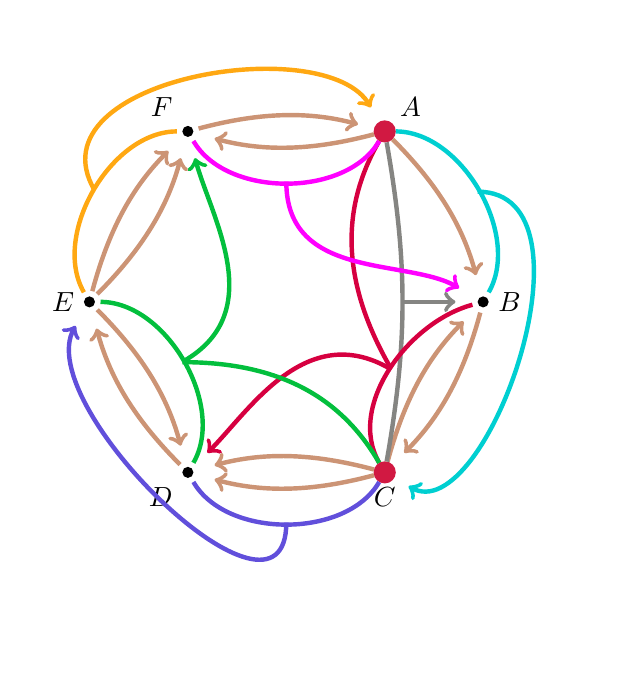
\begin{tikzpicture}
				\def\radius{2.5}
				\coordinate (A) at (60:\radius);
				\coordinate (B) at (0:\radius);
				\coordinate (C) at (300:\radius);
				\coordinate (D) at (240:\radius);
				\coordinate (E) at (180:\radius);
				\coordinate (F) at (120:\radius);
				
				\fill (A) circle (2pt); \node[above right=2pt] at (A) {$A$}; \visible<2->{\fill[alizarin] (A) circle (4pt);}
				\fill (B) circle (2pt); \node[right=2pt] at (B) {$B$};
				\fill (C) circle (2pt); \node[below=2pt] at (C) {$C$}; \visible<2->{\fill[alizarin] (C) circle (4pt);}
				\fill (D) circle (2pt); \node[below left=2pt] at (D) {$D$};
				\fill (E) circle (2pt); \node[left=2pt] at (E) {$E$};
				\fill (F) circle (2pt); \node[above left=2pt] at (F) {$F$};
				
				\visible<-2>{
					\draw[ultra thick, antiquebrass, shorten <= 4pt, shorten >= 10pt, ->] (A) to [out=-45, in=105] (B);
					\draw[ultra thick, antiquebrass, shorten <= 4pt, shorten >= 10pt, ->] (C) to [out=195, in=-15] (D);
					\draw[ultra thick, antiquebrass, shorten <= 4pt, shorten >= 10pt, ->] (D) to [out=135, in=-75] (E);
					\draw[ultra thick, antiquebrass, shorten <= 4pt, shorten >= 10pt, ->] (E) to [out=75, in=-135] (F);
					\draw[ultra thick, antiquebrass, shorten <= 4pt, shorten >= 10pt, ->] (A) to [out=195, in=-15] (F);
					\draw[ultra thick, antiquebrass, shorten <= 4pt, shorten >=10pt, ->] (C) to [out=75, in=-135] (B);
					\draw[ultra thick, antiquebrass, shorten <= 10pt, shorten >= 4pt, <-] (D) to [out=15, in=165] (C);
					\draw[ultra thick, antiquebrass, shorten <= 4pt, shorten >= 10pt, ->] (E) to [out=-45, in=105] (D);
					\draw[ultra thick, antiquebrass, shorten <= 10pt, shorten >= 4pt, <-] (F) to [out=-105, in=45] (E);
				}
				
				\visible<-3>{
					\draw[ultra thick, antiquebrass, shorten <= 4pt, shorten >= 10pt, ->] (B) to [out=-105, in=45] (C);
					\draw[ultra thick, antiquebrass, shorten <= 4pt, shorten >= 10pt, ->] (F) to [out=15, in=165] (A);
				}
				
				\visible<-2>{
					% {AC -> B}
					\draw[ultra thick, battleshipgrey, shorten <= 4pt, shorten >= 4pt] (A) to [out=-80, in=80] node[pos=0.5] (ac)   {} (C);
					\draw[ultra thick, battleshipgrey, shorten <= -4pt, shorten >= 10pt, ->] (ac) to [out = 0, in = 180] (B);
				}
				
				\visible<-3>{
					% {AB -> C}
					\draw[ultra thick, darkturquoise, shorten <= 4pt, shorten >= 4pt] (A) to [out=0, in=60] node[pos=0.5] (ab) {} (B);
					\draw[ultra thick, darkturquoise, shorten <= -4pt, shorten >= 10pt, ->] (ab) to [out = 0, in = -30] (C);
				}
				
				\visible<-2>{
					% {ABC -> D}
					\draw[ultra thick, richcarmine, shorten <= 4pt, shorten >= 4pt] (B) to [out=195, in=120] node[pos=0.5] (bc) {} (C);
					\draw[ultra thick, richcarmine, shorten <= 4pt, shorten >= -4pt] (A) to [out=-120, in=120] (bc);
					\draw[ultra thick, richcarmine, shorten <= -4pt, shorten >= 10pt, ->] (bc) to [out = 150, in = 45] (D);
				}
				
				\visible<-2>{
					% {CD -> E}
					\draw[ultra thick, majorelleblue, shorten <= 4pt, shorten >= 4pt] (C) to [out=240, in=-60] node[pos=0.5] (cd) {} (D);
					\draw[ultra thick, majorelleblue, shorten <= -4pt, shorten >= 10pt, ->] (cd) to [out = -90, in = -120] (E);
				}
				
				\visible<-2>{
					% {CDE -> F}
					\draw[ultra thick, darkpastelgreen, shorten <= 4pt, shorten >= 4pt] (D) to [out=60, in=0] node[pos=0.5] (de) {} (E);
					\draw[ultra thick, darkpastelgreen, shorten <= 4pt, shorten >= -4pt] (C) to [out=120, in=0] (de);
					\draw[ultra thick, darkpastelgreen, shorten <= -4pt, shorten >= 10pt, ->] (de) to [out = 30, in = -75] (F);
				}
				
				\visible<-3>{
					% {EF -> A}
					\draw[ultra thick, darktangerine, shorten <= 4pt, shorten >= 4pt] (E) to [out=120,in=180] node[pos=0.5] (ef) {} (F);
					\draw[ultra thick, darktangerine, shorten <= -4pt, shorten >= 10pt, ->] (ef) to [out = 120, in = 120] (A);
				}
				
				\visible<-2>{
					% {FA -> B}
					\draw[ultra thick, magenta, shorten <= 4pt, shorten >= 4pt] (F) to [out = -60, in = -120] node[pos=0.5] (fa) {} (A);
					\draw[ultra thick, magenta, shorten <= -4pt, shorten >= 10pt, ->] (fa) to [out = -90, in = 150] (B);
				}
			\end{tikzpicture}
		\end{figure}
		
	\end{frame}
	
	\begin{frame}{Out-Degree of $\varnothing\not=\mathsf{X}\subsetneq V$}
		$d^{+}_{\mathcal{H}}(\mathsf{X})$ is the number of hyperarcs $(\mathsf{Y}, v)$ such that $v\not\in\mathsf{X}$ and $\exists u \in \mathsf{Y}\cap\mathsf{X}$.
		\begin{figure}[H]
			\centering
			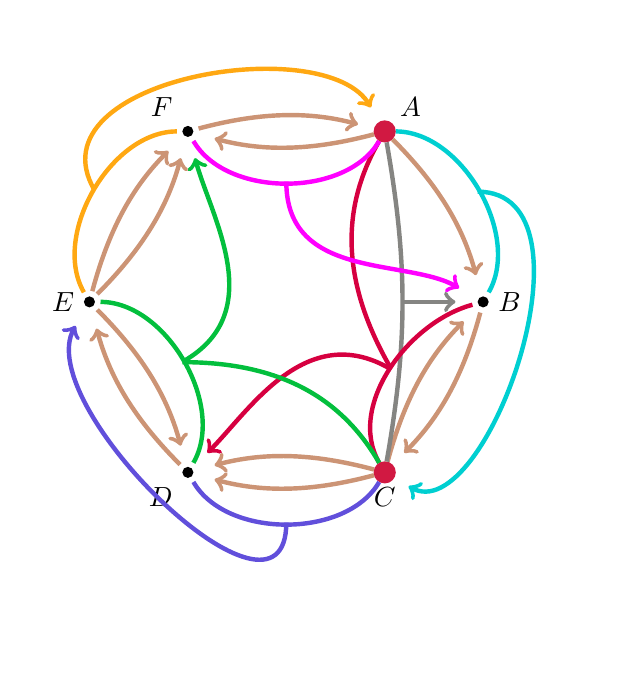
\begin{tikzpicture}
				\def\radius{2.5}
				\coordinate (A) at (60:\radius);
				\coordinate (B) at (0:\radius);
				\coordinate (C) at (300:\radius);
				\coordinate (D) at (240:\radius);
				\coordinate (E) at (180:\radius);
				\coordinate (F) at (120:\radius);
				
				\fill (A) circle (2pt); \node[above right=2pt] at (A) {$A$}; \visible<2->{\fill[alizarin] (A) circle (4pt);}
				\fill (B) circle (2pt); \node[right=2pt] at (B) {$B$};
				\fill (C) circle (2pt); \node[below=2pt] at (C) {$C$}; \visible<2->{\fill[alizarin] (C) circle (4pt);}
				\fill (D) circle (2pt); \node[below left=2pt] at (D) {$D$};
				\fill (E) circle (2pt); \node[left=2pt] at (E) {$E$};
				\fill (F) circle (2pt); \node[above left=2pt] at (F) {$F$};
				
				\visible<-2>{
					\draw[ultra thick, antiquebrass, shorten <= 4pt, shorten >= 10pt, ->] (B) to [out=-105, in=45] (C);
					\draw[ultra thick, antiquebrass, shorten <= 4pt, shorten >= 10pt, ->] (D) to [out=135, in=-75] (E);
					\draw[ultra thick, antiquebrass, shorten <= 4pt, shorten >= 10pt, ->] (E) to [out=75, in=-135] (F);
					\draw[ultra thick, antiquebrass, shorten <= 4pt, shorten >= 10pt, ->] (F) to [out=15, in=165] (A);
					\draw[ultra thick, antiquebrass, shorten <= 4pt, shorten >= 10pt, ->] (E) to [out=-45, in=105] (D);
					\draw[ultra thick, antiquebrass, shorten <= 10pt, shorten >= 4pt, <-] (F) to [out=-105, in=45] (E);
				}
				
				\visible<-3>{
					\draw[ultra thick, antiquebrass, shorten <= 4pt, shorten >= 10pt, ->] (A) to [out=-45, in=105] (B); 
					\draw[ultra thick, antiquebrass, shorten <= 4pt, shorten >= 10pt, ->] (C) to [out=195, in=-15] (D);
					\draw[ultra thick, antiquebrass, shorten <= 4pt, shorten >= 10pt, ->] (A) to [out=195, in=-15] (F);
					\draw[ultra thick, antiquebrass, shorten <= 4pt, shorten >=10pt, ->] (C) to [out=75, in=-135] (B);
					\draw[ultra thick, antiquebrass, shorten <= 10pt, shorten >= 4pt, <-] (D) to [out=15, in=165] (C);
				}
				
				\visible<-3>{
					% {AC -> B}
					\draw[ultra thick, battleshipgrey, shorten <= 4pt, shorten >= 4pt] (A) to [out=-80, in=80] node[pos=0.5]    (ac) {} (C);
					\draw[ultra thick, battleshipgrey, shorten <= -4pt, shorten >= 10pt, ->] (ac) to [out = 0, in = 180] (B);
				}
				
				\visible<-2>{
					% {AB -> C}
					\draw[ultra thick, darkturquoise, shorten <= 4pt, shorten >= 4pt] (A) to [out=0, in=60] node[pos=0.5] (ab) {}   (B);
					\draw[ultra thick, darkturquoise, shorten <= -4pt, shorten >= 10pt, ->] (ab) to [out = 0, in = -30] (C);
				}
				
				\visible<-3>{
					% {ABC -> D}
					\draw[ultra thick, richcarmine, shorten <= 4pt, shorten >= 4pt] (B) to [out=195, in=120] node[pos=0.5] (bc) {} (C);
					\draw[ultra thick, richcarmine, shorten <= 4pt, shorten >= -4pt] (A) to [out=-120, in=120] (bc);
					\draw[ultra thick, richcarmine, shorten <= -4pt, shorten >= 10pt, ->] (bc) to [out = 150, in = 45] (D);
				}
				
				\visible<-3>{
					% {CD -> E}
					\draw[ultra thick, majorelleblue, shorten <= 4pt, shorten >= 4pt] (C) to [out=240, in=-60] node[pos=0.5] (cd)   {} (D);
					\draw[ultra thick, majorelleblue, shorten <= -4pt, shorten >= 10pt, ->] (cd) to [out = -90, in = -120] (E);
				}
				
				\visible<-3>{
					% {CDE -> F}
					\draw[ultra thick, darkpastelgreen, shorten <= 4pt, shorten >= 4pt] (D) to [out=60, in=0] node[pos=0.5] (de) {} (E);
					\draw[ultra thick, darkpastelgreen, shorten <= 4pt, shorten >= -4pt] (C) to [out=120, in=0] (de);
				}
				\draw[ultra thick, darkpastelgreen, shorten <= -4pt, shorten >= 10pt, ->] (de) to [out = 30, in = -75] (F);
				
				\visible<-2>{
					% {EF -> A}
					\draw[ultra thick, darktangerine, shorten <= 4pt, shorten >= 4pt] (E) to [out=120,in=180] node[pos=0.5] (ef) {} (F);
					\draw[ultra thick, darktangerine, shorten <= -4pt, shorten >= 10pt, ->] (ef) to [out = 120, in = 120] (A);
				}
				
				\visible<-3>{
					% {FA -> B}
					\draw[ultra thick, magenta, shorten <= 4pt, shorten >= 4pt] (F) to [out = -60, in = -120] node[pos=0.5] (fa) {} (A);
					\draw[ultra thick, magenta, shorten <= -4pt, shorten >= 10pt, ->] (fa) to [out = -90, in = 150] (B);
				}
				
			\end{tikzpicture}
		\end{figure}
		
	\end{frame}
	
	\begin{frame}{Hyperarc-connectivity and $(k, k)$-partition connected hypergraphs}
		\begin{itemize}
			\item $\vec{\mathcal{H}}$ is \textit{$k$-hyperarc-connected}, if, $\forall\varnothing\not=X\subsetneq V$, $d^{+}_{\vec{\mathcal{H}}}(X) \geq k$.
			\item The hyperarc-connectivity of a hypergraph, denoted $\lambda(\vec{\mathcal{H}})$, is the maximum value of $k$ such that $\vec{\mathcal{H}}$ is \textit{$k$-hyperarc-connected}.
			\visible<2->{\item The previous orientation given was 2-hyperarc-connected. {\visible<3>{There is a 3-hyperarc-connected orientation of such an hypergraph.}}}
		\end{itemize}
		
		\begin{itemize}
			\visible<4->{\item  Let $\mathcal{P}$ be a partition of $V$ :}
			\visible<4->{\item $e_{\mathcal{H}}(\mathcal{P})$ is the number of hyperedges intersecting at least 2 elements of $\mathcal{P}$}
			\visible<5->{\item $\mathcal{H}$ is $(k,k)$-partition-connected, if : \begin{itemize}
					\item $\forall\mathcal{P}, e_{\mathcal{H}}(\mathcal{P}) \geq k \times |\mathcal{P}| $
			\end{itemize}}
		\end{itemize}
		\visible<6->{We use a result of Frank : $\mathcal{H}$ is $(k, k)$-partition-connected if and only if it admits a $k$-hyperarc-connected orientation.}
	\end{frame}
	
	\begin{frame}{Main result}
		\begin{tcolorbox}[colback=bondiblue!5!white,colframe=bondiblue!75!black,title=Main result (Theorem 7)]
			Let $\mathcal{H} = (V, E)$ be a $(k+1, k+1)$-partition-connected hypergraph and $\vec{\mathcal{H}}$ is a k-hyperarc connected orientation of $\mathcal{H}$. Then there exists a sequence of hypergraphs $(\vec{\mathcal{H}_{i}})_{i\in0\dots\ell}$ such that $\vec{\mathcal{H}}_{i+1}$ is obtained from $\vec{\mathcal{H}}_{i}$ by reorienting exactly one hyperarc and $\lambda(\vec{\mathcal{H}}_{i+1}) \geq \lambda(\vec{\mathcal{H}}_{i})$ and $\lambda(\vec{\mathcal{H}}_{\ell}) = k + 1$. Such a sequence of orientations can be obtained with $\ell \leq |V|^{3}$ and found in polynomial time (in the size of $\mathcal{H}$).
		\end{tcolorbox}
		\visible<2->{Generalization of \textbf{Ito and al.}, as digraphs are special cases of hypergraphs.}
	\end{frame}
	
	\begin{frame}{"High-Level"-running of the algorithm}
		Our algorithm will provide a 3-hyperarc-connected orientation of $\mathcal{H}$, starting from a 2-hyperarc-connected.
		
		\begin{columns}
			\begin{column}{0.5\textwidth}
				\begin{figure}[H]
					\centering
					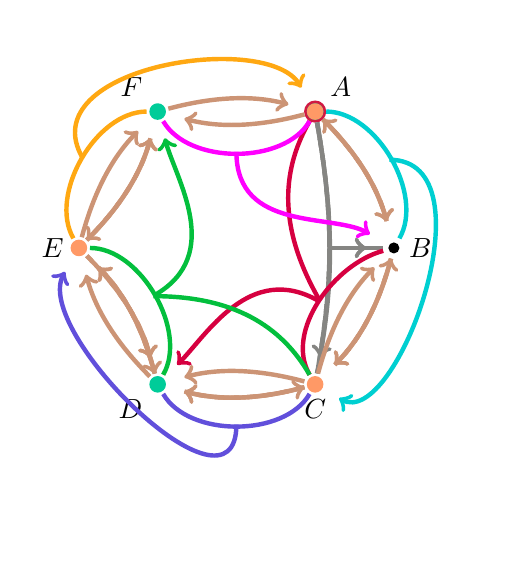
\begin{tikzpicture}
						\def\radius{2}
						\coordinate (A) at (60:\radius);
						\coordinate (B) at (0:\radius);
						\coordinate (C) at (300:\radius);
						\coordinate (D) at (240:\radius);
						\coordinate (E) at (180:\radius);
						\coordinate (F) at (120:\radius);
						
						\fill (A) circle (2pt); \node[above right=2pt] at (A) {$A$}; \visible<2>{\fill[alizarin] (A) circle (4pt);} \visible<5>{\fill[caribbeangreen] (A) circle (3 pt);} \visible<13-18>{\fill[atomictangerine] (A) circle (3 pt);}
						\fill (B) circle (2pt); \node[right=2pt] at (B) {$B$};
						\fill (C) circle (2pt); \node[below=2pt] at (C) {$C$}; \visible<5>{\fill[atomictangerine] (C) circle (3 pt);}
						\fill (D) circle (2pt); \node[below left=2pt] at (D) {$D$}; \visible<9>{\fill[caribbeangreen] (D) circle (3 pt);}
						\fill (E) circle (2pt); \node[left=2pt] at (E) {$E$}; \visible<9>{\fill[atomictangerine] (E) circle (3 pt);}
						\fill (F) circle (2pt); \node[above left=2pt] at (F) {$F$}; \visible<13-18>{\fill[caribbeangreen] (F) circle (3 pt);}
						
						\visible<-12>{
							\draw[ultra thick, antiquebrass, shorten <= 4pt, shorten >= 10pt, ->] (A) to [out=-45, in=105] (B);
						}
						
						\visible<13-17>{
							\draw[dashed, ultra thick, antiquebrass, shorten <= 4pt, shorten >= 10pt, ->] (A) to [out=-45, in=105] (B);
						}
						
						\visible<18->{
							\draw[ultra thick, antiquebrass, shorten <= 4pt, shorten >= 10pt, <-] (A) to [out=-45, in=105] (B);
						}
						
						\visible<-12>{
							\draw[ultra thick, antiquebrass, shorten <= 4pt, shorten >= 10pt, ->] (B) to [out=-105, in=45] (C);
						}
						\visible<13-16>{
							\draw[dashed, ultra thick, antiquebrass, shorten <= 4pt, shorten >= 10pt, ->] (B) to [out=-105, in=45] (C);
						}
						\visible<17->{
							\draw[ultra thick, antiquebrass, shorten <= 4pt, shorten >= 10pt, <-] (B) to [out=-105, in=45] (C);
						}
					
						\visible<-12>{
							\draw[ultra thick, antiquebrass, shorten <= 4pt, shorten >= 10pt, ->] (C) to [out=195, in=-15] (D);
						}
						\visible<13-15>{
							\draw[dashed, ultra thick, antiquebrass, shorten <= 4pt, shorten >= 10pt, ->] (C) to [out=195, in=-15] (D);
						}
						\visible<16->{
							\draw[ultra thick, antiquebrass, shorten <= 4pt, shorten >= 10pt, <-] (C) to [out=195, in=-15] (D);
						}
					
						\draw[ultra thick, antiquebrass, shorten <= 4pt, shorten >= 10pt, ->] (D) to [out=135, in=-75] (E);
						\draw[ultra thick, antiquebrass, shorten <= 4pt, shorten >= 10pt, ->] (E) to [out=75, in=-135] (F);
						\draw[ultra thick, antiquebrass, shorten <= 4pt, shorten >= 10pt, ->] (F) to [out=15, in=165] (A);
						\draw[ultra thick, antiquebrass, shorten <= 4pt, shorten >= 10pt, ->] (A) to [out=195, in=-15] (F);
						
						\visible<-4>{
							% {AC -> B}
							\draw[ultra thick, battleshipgrey, shorten <= 4pt, shorten >= 4pt] (A) to [out=-80, in=80] node[pos=0.5] (ac) {} (C);
							\draw[ultra thick, battleshipgrey, shorten <= -4pt, shorten >= 10pt, ->] (ac) to [out = 0, in = 180] (B);
						}
						\visible<5>{
							% {AC -> B}
							\draw[dashed, ultra thick, battleshipgrey, shorten <= 4pt, shorten >= 4pt] (A) to [out=-80, in=80] node[pos=0.5] (ac) {} (C);
							\draw[dashed, ultra thick, battleshipgrey, shorten <= -4pt, shorten >= 10pt, ->] (ac) to [out = 0, in = 180] (B);
						}
						\visible<6->{
							% {AB -> C}
							\draw[ultra thick, battleshipgrey, shorten <= 4pt, shorten >= 10pt, ->] (A) to [out=-80, in=80] node[pos=0.5] (ac) {} (C);
							\draw[ultra thick, battleshipgrey, shorten <= -4pt, shorten >= 4pt] (ac) to [out = 0, in = 180] (B);
						}
						
						\draw[ultra thick, antiquebrass, shorten <= 4pt, shorten >=10pt, ->] (C) to [out=75, in=-135] (B);
						\draw[ultra thick, antiquebrass, shorten <= 10pt, shorten >= 4pt, <-] (D) to [out=15, in=165] (C);
						
						\visible<-8>{
							\draw[ultra thick, antiquebrass, shorten <= 4pt, shorten >= 10pt, ->] (E) to [out=-45, in=105] (D);
						}
						\visible<9>{
							\draw[dashed, ultra thick, antiquebrass, shorten <= 4pt, shorten >= 10pt, ->] (E) to [out=-45, in=105] (D);
						}
						\visible<10-12>{
							\draw[ultra thick, antiquebrass, shorten <= 10pt, shorten >= 4pt, <-] (E) to [out=-45, in=105] (D);
						}
						\visible<13-14>{
							\draw[dashed, ultra thick, antiquebrass, shorten <= 10pt, shorten >= 4pt, <-] (E) to [out=-45, in=105] (D);
						}
						\visible<15->{
							\draw[ultra thick, antiquebrass, shorten <= 10pt, shorten >= 4pt, ->] (E) to [out=-45, in=105] (D);
						}
						
						\visible<-12>{
							\draw[ultra thick, antiquebrass, shorten <= 10pt, shorten >= 4pt, <-] (F) to [out=-105, in=45] (E);
						}
						\visible<13>{
							\draw[dashed, ultra thick, antiquebrass, shorten <= 10pt, shorten >= 4pt, <-] (F) to [out=-105, in=45] (E);
						}
						\visible<14->{
							\draw[ultra thick, antiquebrass, shorten <= 10pt, shorten >= 4pt, ->] (F) to [out=-105, in=45] (E);
						}
						
						% {AB -> C}
						\draw[ultra thick, darkturquoise, shorten <= 4pt, shorten >= 4pt] (A) to [out=0, in=60] node[pos=0.5] (ab) {} (B);
						\draw[ultra thick, darkturquoise, shorten <= -4pt, shorten >= 10pt, ->] (ab) to [out = 0, in = -30] (C);
						
						% {ABC -> D}
						\draw[ultra thick, richcarmine, shorten <= 4pt, shorten >= 4pt] (B) to [out=195, in=120] node[pos=0.5] (bc) {} (C);
						\draw[ultra thick, richcarmine, shorten <= 4pt, shorten >= -4pt] (A) to [out=-120, in=120] (bc);
						\draw[ultra thick, richcarmine, shorten <= -4pt, shorten >= 10pt, ->] (bc) to [out = 150, in = 45] (D);
						
						% {CD -> E}
						\draw[ultra thick, majorelleblue, shorten <= 4pt, shorten >= 4pt] (C) to [out=240, in=-60] node[pos=0.5] (cd) {} (D);
						\draw[ultra thick, majorelleblue, shorten <= -4pt, shorten >= 10pt, ->] (cd) to [out = -90, in = -120] (E);
						
						% {CDE -> F}
						\draw[ultra thick, darkpastelgreen, shorten <= 4pt, shorten >= 4pt] (D) to [out=60, in=0] node[pos=0.5] (de) {} (E);
						\draw[ultra thick, darkpastelgreen, shorten <= 4pt, shorten >= -4pt] (C) to [out=120, in=0] (de);
						
						\draw[ultra thick, darkpastelgreen, shorten <= -4pt, shorten >= 10pt, ->] (de) to [out = 30, in = -75] (F);
						
						% {EF -> A}
						\draw[ultra thick, darktangerine, shorten <= 4pt, shorten >= 4pt] (E) to [out=120,in=180] node[pos=0.5] (ef) {} (F);
						\draw[ultra thick, darktangerine, shorten <= -4pt, shorten >= 10pt, ->] (ef) to [out = 120, in = 120] (A);
						
						% {FA -> B}
						\draw[ultra thick, magenta, shorten <= 4pt, shorten >= 4pt] (F) to [out = -60, in = -120] node[pos=0.5] (fa) {} (A);
						\draw[ultra thick, magenta, shorten <= -4pt, shorten >= 10pt, ->] (fa) to [out = -90, in = 150] (B);
						
					\end{tikzpicture}
				\end{figure}
			\end{column}
			\hfill
			\begin{column}{0.5\textwidth}
				\begin{enumerate}
					\item <alert@2> Take $r$ in $V(\mathcal{H})$.
					\item <alert@3,7,11,19> Compute sets of vertices.
					\item <alert@20> Stopping Criteria
					\item <alert@4,8,12> Select a set $R$ (cf. 2.)
					\item <alert@5,9,13> \textbf<21>{Find an admissible $(s, t)$-hyperpath in $R$ to reorient}
					\item <alert@6,10,14-18> Reorient the corresponding hyperpath.
					\item <alert@7,11,19> \texttt{Goto} (2.)
				\end{enumerate}
			\end{column}
		\end{columns}
		\visible<21>{We consider until the end of the presentation $r\in{V}$ fixed.}	
	\end{frame}

	\begin{frame}{Finding \textit{admissible} $(s, t)$-hyperpaths in $R$}
		\begin{itemize}
			\item<1-> Crucial segment of the algorithm.
			\item<2-> Three criterion for $P$ to be an admissible $(s, t)$-hyperpath in $R$:
			\begin{enumerate}
				\item<3-> $s$ is a {\color<4->{alizarin}safe source} in $S\subseteq{R}$, $t$ is a {\color<4->{alizarin}safe sink} in $T\subseteq{R}$.
				\item<5-> Reorient each hyperarc, \textbf{one by one}, does not decrease the hyperarc-connectivity.
				\item<6-> After reorientation of $P$, there is a set whose cardinality is a guarantee that the algorithm will stop.
			\end{enumerate}
		\end{itemize}

		\visible<7->{What are {\color{alizarin}safe sources} and {\color{alizarin}safe sinks} ?\\
		\begin{flushright}
			\textit{A brief detour...}
		\end{flushright}}
	\end{frame}

	\begin{frame}{Tight and Dangerous sets}
		\only<1>{
			Remainder of the algorithm :
			\begin{itemize}
				\item<1->\texttt{Input} : A $k$-hyperarc-connected orientation of a $(k+1, k+1)$-partition-connected hypergraph.\\
				\item<1->\texttt{Output} : A $k+1$-hyperarc-connected hypergraph.
			\end{itemize}
		}

		\visible<2->{
			\begin{columns}
				\begin{column}{0.45\textwidth}
					\begin{figure}[H]
						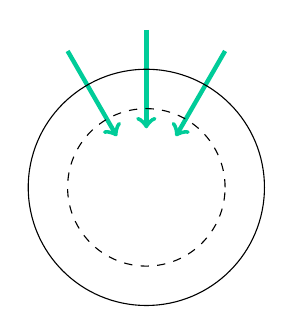
\begin{tikzpicture}
							\def\radius{0.75}
							\def\smol{1}
							\def\mid{1.5}
							\def\Radius{2}

							\coordinate (u) at (120:\radius);
							\coordinate (U) at (120:\Radius);

							\coordinate (v) at (90:\radius);
							\coordinate (V) at (90:\Radius);

							\coordinate (w) at (60:\radius);
							\coordinate (W) at (60:\Radius);
						
							\draw[ultra thick, ->, caribbeangreen] (U) to [out=-60, in=120] (u);
							\visible<3>{\draw[ultra thick, ->, caribbeangreen] (V) to [out=-90, in=90] (v);}
							\draw[ultra thick, ->, caribbeangreen] (W) to [out=-120, in=60] (w);
							
							\visible<-5>{\draw[thin] (0,0) circle (\mid);}
							\visible<5->{\draw[thin, dashed] (0,0) circle (\smol);}
										
						\end{tikzpicture}

						\caption*{\only<5->{Minimal }In-\only<2,4->{Tight}\only<3>{Dangerous} sets}
					\end{figure}
				\end{column}
				\hfill\vrule\hfill
				\begin{column}{0.45\textwidth}
					\begin{figure}[H]
						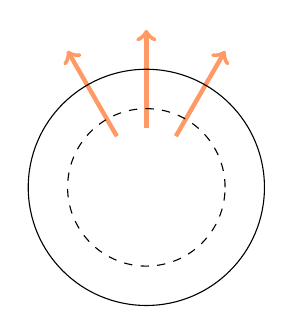
\begin{tikzpicture}
							\def\radius{0.75}
							\def\smol{1}
							\def\mid{1.5}
							\def\Radius{2}

							\coordinate (u) at (120:\radius);
							\coordinate (U) at (120:\Radius);

							\coordinate (v) at (90:\radius);
							\coordinate (V) at (90:\Radius);

							\coordinate (w) at (60:\radius);
							\coordinate (W) at (60:\Radius);
						
							\draw[ultra thick, <-, atomictangerine] (U) to [out=-60, in=120] (u);
							\visible<3>{\draw[ultra thick, <-, atomictangerine] (V) to [out=-90, in=90] (v);}
							\draw[ultra thick, <-, atomictangerine] (W) to [out=-120, in=60] (w);
							
							\visible<-5>{\draw[thin] (0,0) circle (\mid);}
							\visible<5->{\draw[thin, dashed] (0,0) circle (\smol);}				
						\end{tikzpicture}
						\caption*{\only<5->{Minimal }Out-\only<2,4->{Tight}\only<3>{Dangerous} sets}
					\end{figure}
				\end{column}
			\end{columns}
		}

		\only<2->{
			\begin{itemize}
				\item ${\color{caribbeangreen}\mathcal{T}_{-}} = \{X \subseteq V - r, d^{-}(X) = k\} \cup \{V\}$
				\item ${\color{atomictangerine}\mathcal{T}_{+}} = \{X \subseteq V - r, d^{+}(X) = k\} \cup \{V\}$
				\item<3> ${\color{caribbeangreen}\mathcal{D}_{-}} = \{X \subseteq V - r, d^{-}(X) = k + 1\}$ 
				\item<3> ${\color{atomictangerine}\mathcal{D}_{+}} = \{X \subseteq V - r, d^{+}(X) = k + 1\}$
				\item<5-> ${\color{caribbeangreen}\mathcal{M}_{-}}$ : Inclusion-wise minimal members of ${\color{caribbeangreen}\mathcal{T}_{-}}$
				\item<5-> ${\color{atomictangerine}\mathcal{M}_{+}}$ : Inclusion-wise minimal members of ${\color{atomictangerine}\mathcal{T}_{+}}$
				\item<5-> $\mathcal{M}$ : Inclusion-wise minimal members of $\mathcal{M}_{-}\cup\mathcal{M}_{+}$
			\end{itemize}
		}

	\end{frame}

	\begin{frame}{Crossing sets and structural results}
		Let $X, Y$ two crossing sets in $V$.
		\begin{block}{Claim 1(b)}
			If $X, Y\in{\color{atomictangerine}\mathcal{T}_{+}}$, then both $X\cup{Y}\in{\color{atomictangerine}\mathcal{T}_{+}}$ and $X\cap{Y}\in{\color{atomictangerine}\mathcal{T}_{+}}$.
		\end{block}
		\only<2->{
			\begin{block}{Proof of Claim 1(b)}
				\begin{itemize}[<+->]
					\item We have $\lambda(\vec{\mathcal{H}}) = k$
					\item Since $X, Y$ are crossing, $X\cap{Y}\not=\varnothing$, $X\cup{Y}\not=V$.
					\item $k + k = d^{+}(X) + d^{+}(Y)$
					\item By submodularity, $d^{+}(X) + d^{+}(Y) \geq d^{+}(X\cup{Y}) + d^{+}(X\cap{Y})$
					\item By $\lambda(\vec{\mathcal{H}}) = k$, $d^{+}(X\cup{Y}) \geq k$ and $d^{+}(X\cap{Y}) \geq k$
					\item Grouping these equations, we obtain : $k + k = d^{+}(X) + d^{+}(Y) \geq d^{+}(X\cup{Y}) + d^{+}(X\cap{Y}) \geq k + k$.
					\item This implies $d^{+}(X\cup Y) = k$, $d^{+}(X\cap Y)$, i.e. $X\cap Y, X\cup Y \in {\color{atomictangerine}\mathcal{T}_{+}}$
				\end{itemize}
			\end{block}
		}
	\end{frame}

	\mode<handout>{
		\begin{frame}{Safe Sources and Safe Sinks}
			Definitions are symmetric (but proofs are not).
			\only<1-2>{\begin{itemize}
				\item For $S \in \mathcal{M}_{-}$, $s$ is a safe source in $S$ if :\begin{itemize}
					\item[a]<1,2>{For every $s\in{X}\in\mathcal{T}_{+}$, we have $\color{red} S\subsetneq X$.}
					\item[b]<2>{For every $s\in{X}\in\mathcal{D}_{+}$ such that $S\setminus{X}\not=\varnothing$, there exists $Y\in\mathcal{T}_{+}$ such that $s\not\in{Y}\subsetneq{X}$.}
				\end{itemize}
			\end{itemize}
			\begin{columns}
				\begin{column}{0.35\textwidth}
					\only<1,2>{
						\begin{figure}[H]
							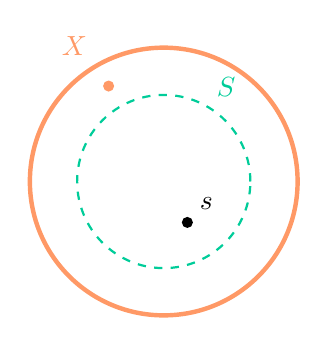
\begin{tikzpicture}
								\def\smolrad{0.6}
								\def\midrad{1.1}
								\def\intrad{1.4}
								\def\bigrad{1.7}

								\coordinate (s) at (-60:\smolrad);
								\fill (s) circle (2pt);
								\node[above right=1pt] at (s) {$s$};

								\coordinate (S) at (60:\midrad);
								\node[above right] at (S) {$\color{caribbeangreen}S$};

								\coordinate (X) at (120:\bigrad);
								\node[above left] at (X) {$\color{atomictangerine}{X}$};

								\coordinate (x) at (120:\intrad);
								\fill[atomictangerine] (x) circle (2pt);

								\draw[thick, caribbeangreen, dashed] (0,0) circle (\midrad);
								\draw[ultra thick, atomictangerine] (0,0) circle (\bigrad);
							\end{tikzpicture}
							\caption*{Condition (a)}
						\end{figure}
					}
				\end{column}
				\hfill\vrule\hfill
				\begin{column}{0.60\textwidth}
					\only<2>{
						\begin{figure}[H]
							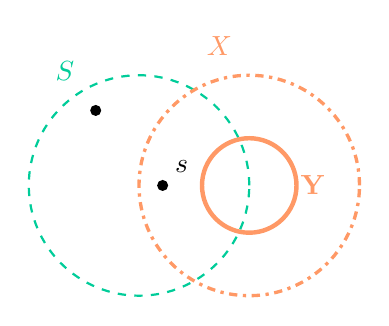
\begin{tikzpicture}
								\def\ssmolrad{0.3}
								\def\smolrad{0.6}
								\def\midrad{1.1}
								\def\intrad{1.4}
								\def\bigrad{1.7}

								\coordinate (s) at (0:\ssmolrad);
								\fill (s) circle (2pt);
								\node[above right=1pt] at (s) {$s$};

								\coordinate (S) at (120:\intrad);
								\node[above left] at (S) {$\color{caribbeangreen}S$};

								\fill(120:\midrad) circle (2pt);

								\node at (60:{1.2*\bigrad}) {$\color{atomictangerine}X$};
								\node at (0:{1.3*\bigrad}) {$\color{atomictangerine}\mathbf{Y}$};
								
								\draw[thick, caribbeangreen, dashed] (0,0) circle (\intrad);

								\coordinate (cE) at (0:\intrad);
								\draw[very thick, atomictangerine, dashdotted] (cE) circle (\intrad);
								\draw[ultra thick, atomictangerine] (cE) circle (\smolrad);
							\end{tikzpicture}
							\caption*{Condition (b)}
						\end{figure}
					}
				\end{column}
			\end{columns}
			}
			\only<3>{\begin{itemize}
				\item For $T \in \mathcal{M}_{+}$, $t$ is a safe sink in $T$ if :\begin{itemize}
					\item[c]{For every $t\in{X}\in\mathcal{T}_{-}$, we have $\color{red}T\subsetneq X$.}
					\item[d]{For every $t\in{X}\in\mathcal{D}_{-}$ such that $T\setminus{X}\not=\varnothing$, there exists $Y\in\mathcal{T}_{-}$ such that $t\not\in{Y}\subsetneq{X}$.}
				\end{itemize}
			\end{itemize}
			\begin{columns}
				\begin{column}{0.35\textwidth}
					\begin{figure}[H]
						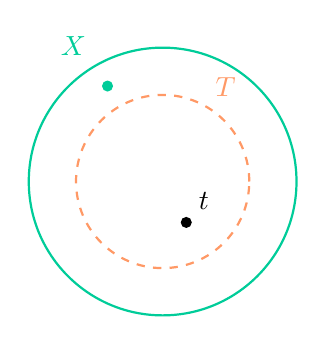
\begin{tikzpicture}
							\def\smolrad{0.6}
							\def\midrad{1.1}
							\def\intrad{1.4}
							\def\bigrad{1.7}

							\coordinate (t) at (-60:\smolrad);
							\fill (t) circle (2pt);
							\node[above right=1pt] at (t) {$t$};

							\coordinate (T) at (60:\midrad);
							\node[above right] at (T) {$\color{atomictangerine}T$};

							\coordinate (X) at (120:\bigrad);
							\node[above left] at (X) {$\color{caribbeangreen}{X}$};

							\coordinate (x) at (120:\intrad);
							\fill[caribbeangreen] (x) circle (2pt);

							\draw[thick, atomictangerine, dashed] (0,0) circle (\midrad);
							\draw[thick, caribbeangreen] (0,0) circle (\bigrad);
						\end{tikzpicture}
						\caption*{Condition (c)}
					\end{figure}
				\end{column}
				\hfill\vrule\hfill
				\begin{column}{0.60\textwidth}
					\begin{figure}[H]
						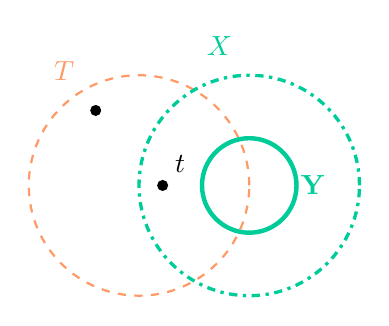
\begin{tikzpicture}
							\def\ssmolrad{0.3}
							\def\smolrad{0.6}
							\def\midrad{1.1}
							\def\intrad{1.4}
							\def\bigrad{1.7}

							\coordinate (t) at (0:\ssmolrad);
							\fill (t) circle (2pt);
							\node[above right=1pt] at (t) {$t$};

							\coordinate (T) at (120:\intrad);
							\node[above left] at (T) {$\color{atomictangerine}T$};

							\fill(120:\midrad) circle (2pt);

							\node at (60:{1.2*\bigrad}) {$\color{caribbeangreen}X$};
							\node at (0:{1.3*\bigrad}) {$\color{caribbeangreen}\mathbf{Y}$};
							
							\draw[thick, atomictangerine, dashed] (0,0) circle (\intrad);

							\coordinate (cE) at (0:\intrad);
							\draw[very thick, caribbeangreen, dashdotted] (cE) circle (\intrad);
							\draw[ultra thick, caribbeangreen] (cE) circle (\smolrad);
						\end{tikzpicture}
						\caption*{Condition (d)}
					\end{figure}
				\end{column}
			\end{columns}
			}
			Finding a safe sink $t$ in $T\in\mathcal{M}_{+}$ can be done by checking each vertex if they correspond to the definition.
		\end{frame}
	}

	\begin{frame}{Existence of a safe source (\textit{a safe sink})}
		\begin{block}{Lemma 10}$\forall{S}\in\mathcal{M}_{-}, \text{ there is a safe source }s\in{S}.$\end{block}
		Likewise,
		\begin{block}{Lemma 11}$\forall{T}\in\mathcal{M}_{+}, \text{ there is a safe sink }t\in{T}.$\end{block}

		\begin{block}
			{Quick outline of a proof for \textsf{Lemma 10} :}
			\begin{itemize}
				\item Let $S\in\mathcal{M}_{-}$.
				\item Considering a family of vertex sets ($\chi$) that cover as many vertices of $S$ as possible, but using as little as vertex sets possible.
				\item We can prove that, under given assumptions, $\chi$ cannot cover every vertex of $S$.
				\item Vertices that are not covered by $\chi$ are "potential" safe sources, the last part of the proof is verifying that they are effectively safe sources.
			\end{itemize}
		\end{block}
	\end{frame}

	\begin{frame}{Towards hyperarc connectivity augmentation}
		$\mathcal{R}$ : $R\subseteq V - r$ inclusion-wise minimal such that either :
		\begin{itemize}
			\item $R\in{\color{caribbeangreen}\mathcal{T}_{-}}$, and contains a member of ${\color{atomictangerine}\mathcal{T}_{+}}$
			\item or $R\in{\color{atomictangerine}\mathcal{T}_{+}}$, and contains a member of ${\color{caribbeangreen}\mathcal{T}_{-}}$.
		\end{itemize}
		\visible<2->{
			\begin{block}{Lemma 13}
				Let $R\in\mathcal{R}, S\in{\color{caribbeangreen}\mathcal{M}_{-}}, T\in{\color{atomictangerine}\mathcal{M}_{+}}$ such that $S,T\subseteq{R}$. Let $s$ be a safe source in $S$, $t$ a safe sink in $T$.\\
				Then :
				\begin{itemize}
					\item $\forall{X}\subseteq V-r$ such that $s\in X$, $t\not\in X$, we have $d^{+}(X) \geq k + 1$.
					\item $\forall{X}\subseteq V-r$ such that $s\not\in X$, $t\in X$, we have $d^{-}(X) \geq k + 1$.
				\end{itemize}
			\end{block}
		}
		% TODO
	\end{frame}

	\begin{frame}{Towards hyperarc connectivity augmentation - Proof}
		\only<1>{\begin{block}{Lemma 13}
			Let $R\in\mathcal{R}, S\in{\color{caribbeangreen}\mathcal{M}_{-}}, T\in{\color{atomictangerine}\mathcal{M}_{+}}$ such that $S,T\subseteq{R}$. Let $s$ be a safe source in $S$, $t$ a safe sink in $T$.\\
			Then :
			\begin{itemize}
				\item $\forall{X}\subseteq V-r$ such that $s\in X$, $t\not\in X$, we have $d^{+}(X) \geq k + 1$.
				\item $\forall{X}\subseteq V-r$ such that $s\not\in X$, $t\in X$, we have $d^{-}(X) \geq k + 1$.
			\end{itemize}
		\end{block}}
		\only<2->{
			\begin{block}{Proof of Lemma 13}
				By contradiction, either :
				\begin{itemize}
					\item[a.] $s\in X, t\not\in X, d^{+}(X) = k$, i.e. $s\in X, t\not\in X, X\in{\color{atomictangerine}\mathcal{T}_{+}}$.{\begin{itemize}
						\item[\only<-3>{a1.}\only<4->{\cancel{a1.}}] $R\in\mathcal{R}\cap{\color{caribbeangreen}\mathcal{T}_{-}}$
						\item[\only<-4>{a2.}\only<5->{\cancel{a2.}}] $R\in\mathcal{R}\cap{\color{atomictangerine}\mathcal{T}_{+}}$ 
					\end{itemize}}
					\item[b.] $s\not\in X, t\in X, d^{-}(X) = k$, i.e. $s\not\in X, t\in X, X\in{\color{caribbeangreen}\mathcal{T}_{-}}$.{\begin{itemize}
						\item[\only<-5>{b1.}\only<6->{\cancel{b1.}}] $R\in\mathcal{R}\cap{\color{caribbeangreen}\mathcal{T}_{-}}$
						\item[\only<-5>{b2.}\only<6->{\cancel{b2.}}] $R\in\mathcal{R}\cap{\color{atomictangerine}\mathcal{T}_{+}}$ 
					\end{itemize}}
				\end{itemize}
			\end{block}
			\begin{itemize}
				\item By {\color{alizarin}definition of a safe source}, $S\subsetneq X$.
				\item By $t\in R\setminus X, R\in \mathcal{R}$, we have $X\not\subseteq R$, which implies $X\setminus R \not= \varnothing$.
			\end{itemize}
		}
		\only<3>{{\color{majorelleblue} a1} : If $R\in\mathcal{R}\cap{\color{caribbeangreen}\mathcal{T}_{-}}$ :
			\begin{itemize}
				\item By using \textsf{Claim 1} on $X\in{\color{atomictangerine}\mathcal{T}_{+}}$ and on $R\in{\color{caribbeangreen}\mathcal{T}_{-}}$, we get $R\setminus X\in{\color{caribbeangreen} \mathcal{T}_{-}}$.
				\item If $X\cap T\not=\varnothing${\begin{itemize}
					\item $X\cap T \in {\color{atomictangerine} \mathcal{T}_{+}}$ , $T$ is no longer minimal, which is a contradiction.
				\end{itemize}}
				\item Hence $X\cap T=\varnothing$, and $T\subseteq R\setminus X$.
				\item $R$ is not minimal, which is a contradiction.
			\end{itemize}
		}
		\only<4>{{\color{majorelleblue} a2} : If $R\in\mathcal{R}\cap{\color{atomictangerine}\mathcal{T}_{+}}$ :
			\begin{itemize}
				\item By using \textsf{Claim 1} on $X, R$, we get $X\cap R\in{\color{atomictangerine}\mathcal{T}_{+}}$
				\item $S\subseteq R\cap X$, $t\in R\setminus X$ suffice to show that $R\cap X \in \mathcal{R}$, with $R\setminus X\subsetneq R$, as $t\in R\setminus X$.
				\item This contradicts that $R\in\mathcal{R}$.
			\end{itemize}
		}

	\end{frame}

	\begin{frame}{Finding \textit{admissible} $(s, t)$-hyperpaths in $R\in\mathcal{R}$}
		Three criterion for $P$ to be an admissible $(s, t)$-hyperpath in $R$:	
		\begin{itemize}
			\item[1.] $s$ is a safe source in $S\subseteq{R}$, $t$ is a safe sink in $T\subseteq{R}$.
			\item[2.] Reorienting each hyperarc, \textbf{one by one}, does not decrease the hyperarc-connectivity
			\item[3.] Let $\vec{\mathcal{H}'}$ the hypergraph obtained after reorientation of $P$.\begin{itemize}
				\item $\mathcal{M}'$ : Inclusion-wise minimal members of $\mathcal{M}'_{-}\cup\mathcal{M}'_{+}$
				\item Either $|\mathcal{M}'| < |\mathcal{M}|$, either $|\mathcal{M}'| = |\mathcal{M}|$ and $\mathcal{M}'$ covers more vertices than $\mathcal{M}$.
			\end{itemize}
		\end{itemize}
		\ \newline
		Point {\color{majorelleblue}3.} is the stopping criteria for the main algorithm :
		\begin{itemize}
			\item $\mathcal{M} = \{V\}$ implies both ${\color{caribbeangreen}\mathcal{M}_{-}} = \{V\}$ and ${\color{atomictangerine}\mathcal{M}_{+}} = \{V\}$.
			\item ${\color{caribbeangreen}\mathcal{T}_{-}} = \{X \subseteq V - r, d^{-}(X) = k\} \cup \{V\}$
			\item ${\color{caribbeangreen}\mathcal{M}_{-}}$ : Inclusion-wise minimal members of ${\color{caribbeangreen}\mathcal{T}_{-}}$
			\item Finally, if $\lambda(\vec{\mathcal{H}}) \geq k$ and ${\color{caribbeangreen}\mathcal{T}_{-}} = {\color{atomictangerine}\mathcal{T}_{+}} = \{V\}$, $\vec{\mathcal{H}}$ is $(k+1)$-hyperarc-connected.
		\end{itemize}
	\end{frame}

	\begin{frame}{Introduction of $Q^{v}_{+}$}
		\begin{block}{Definition of $Q^{v}_{+}$}
			Consider the sets of $\T_{+}$ containing $v$. $Q^{v}_{+}$ is \textbf{the} minimal (inclusion-wise) one.
		\end{block}

		\begin{block}{Unicity of $Q^{v}_{+}$ :}
			If it exists, $Q^{v}_{+}$ is unique.
		\end{block}

		\begin{figure}[H]
			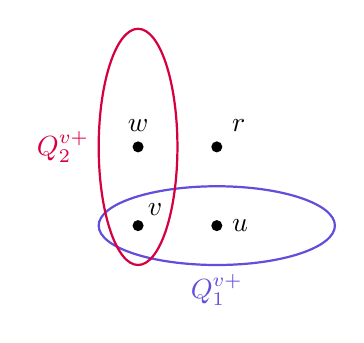
\begin{tikzpicture}
				\coordinate (O) at (0, 0);
				\fill (O) circle (2pt);
				\node[above right] at (O) {$v$};

				\coordinate (X) at (1, 0);
				\node[below = 5mm] at (X) {$\color{majorelleblue} Q^{v+}_{1}$};
				\visible<3->{
					\fill (X) circle (2pt);
					\node[right = 2pt] at (X) {$u$};
				}
				

				\coordinate (Y) at (0, 1);
				\node[left = 5mm] at (Y) {$\color{richcarmine} Q^{v+}_{2}$};
				\visible<3->{
					\fill (Y) circle (2pt);
					\node[above = 2pt] at (Y) {$w$};
				}

				\coordinate (r) at (1, 1);
				\fill (r) circle (2pt);
				\node[above right = 2pt] at (r) {$r$};


				\draw[majorelleblue, thick] (X) ellipse (15mm and 5mm);
				\draw[richcarmine, thick] (Y) ellipse (5mm and 15mm);
			\end{tikzpicture}
			\caption*{
				\only<1>{Let $Q^{v+}_{1}$, $Q^{v+}_{2}$ verifying the above definition.}
				\only<2>{By definition, $Q^{v+}_{1}\not\subseteq Q^{v+}_{2}$ and $Q^{v+}_{2}\not\subseteq Q^{v+}_{1}$.}
				\only<3>{Denote $u\in Q^{v+}_{1}\setminus Q^{v+}_{2}$, $w\in Q^{v+}_{2}\setminus Q^{v+}_{1}$.}
				\only<4>{As $r\not\in Q^{v+}_{1}, Q^{v+}_{2}$, both are are crossing sets.}
				\only<5>{By submodularity, if $X, Y \in {\color{atomictangerine}\mathcal{T}_{+}}$, both $X\cup{V}\in{\color{atomictangerine}\mathcal{T}_{+}}$ and $X\cap{V}\in{\color{atomictangerine}\mathcal{T}_{+}}$.}
				\only<6>{$Q^{v+}_{1}\cap Q^{v+}_{2}$ is smaller (inclusion-wise) than $Q^{v+}_{1}$ and $Q^{v+}_{2}$.}
			}
		\end{figure}
	\end{frame}

	\begin{frame}{Existence of an hyperpath that does not leave $Q^{v}_{+}$}
		\begin{block}{Lemma 12 (a)}
			$\forall{s}\in V, \forall{t}\in Q^{s}_{+}$, there exists an $(s, t)$-hyperpath that does not leave $Q^{s}_{+}$.
		\end{block}

		\begin{block}{Proof of Lemma 12 (a)}
			\begin{itemize}[<+->]
				\item By contradiction, assume that there is $s\in{V}, t\in Q^{s}_{+}$ such that any $(s, t)$-hyperpath leaves $Q^{s}_{+}$.
				\item There is $s\in Z\subseteq Q^{s}_{+}\setminus\{t\}$ such that any hyperarc leaving $Z$ will also leave $Q^{s}_{+}$.
				\item We have the following inequalities{\begin{itemize}[<+->]
					\item $d_{\vec{\mathcal{H}}}^{+}(Q^{s}_{+}) \geq d_{\vec{\mathcal{H}}}^{+}(Z)$
					\item $d_{\vec{\mathcal{H}}}^{+}(Z) \geq k$, as $\mathcal{H}$ is $k$-hyperarc-connected.
					\item $k = d_{\vec{\mathcal{H}}}^{+}(Q^{s}_{+})$ by definition.
				\end{itemize}}
				\item We can deduce that $d_{\vec{\mathcal{H}}}^{+}(Z) = k$, which automatically implies that $Z\in{\color{atomictangerine}\mathcal{T}_{+}}$.
				\item $Q^{s}_{+}$ is not minimal, hence the contradiction.
			\end{itemize}
		\end{block}
	\end{frame}

	\begin{frame}[fragile]{Finding an admissible $(s, t)$-hyperpath in $R\in\mathcal{R}\cap{\color{caribbeangreen}\mathcal{T}_{-}}$}
		\only<-7>{
			\begin{itemize}[<+->]
				\item[1.] Only input of the algorithm $R\in\mathcal{R}\in{\color{caribbeangreen}\mathcal{T}_{-}}${\begin{itemize}
					\item $s, t$ are constrained (maybe not unique) by the choice of $R$.
				\end{itemize}}

				\item[2.] Choosing $S\in{\color{caribbeangreen}\mathcal{M}_{-}}$, then a safe source $s\in S$.
				\item[3.] Main part of the algorithm : $s$-out arborescence{\begin{itemize}
					\item $F$ : (Directed) arborescence, rooted in $s$
					\item $Z$ : Explored (yet) vertices
					\item $V'$ : Allowed remaining vertices to explore
				\end{itemize}}
			\end{itemize}
		}
		\only<8->{
			\begin{algorithm}[H]
				\begin{algorithmic}[1]
					\caption{Admissible $(s, t)$-hyperpath in $R\in\mathcal{R}\cap{\color{caribbeangreen}\mathcal{T}_{-}}$}
					\State{Take a set $S\in{\color{caribbeangreen}\mathcal{M}_{-}}$, with $S\subseteq{R}$, then a safe source $s\in S$.}
					\State{$Z = \{s\}$, $F = (Z, \varnothing)$, $V' = R$}
					\While{$h = (X, v)$ exists such that $v\in V' - Z$ and $X\cap Z\not=\varnothing$}
						\State Let $u\in X\cap{Z}$.
						\State $Z \leftarrow Z\cup\{v\}$
						\State $F \leftarrow F + uv$
						\If{$Q^{v}_{+}\subsetneq V'$}
							\State $V' \leftarrow Q^{v}_{+}$
						\EndIf
					\EndWhile
					\State $T = V'$
					\State Take a safe sink $t\in T$
					\State $P' = F[s, t]$
					\State $P$ is the corresponding hypergraph in $\vec{\mathcal{H}}$ with respect to $P'$.
					\State \textbf{\textsf{Return}} $S, T, s, t, P$
				\end{algorithmic}
				\label{alg_1}
			\end{algorithm}
		}
	\end{frame}

\end{document}